В данном разделе указаны минимальные системные требования. Описан используемый язык и среда разработки.
Представлено описание интерфейса и его скриншоты. Приведен листинг 3 алгоритмов умножения матрицы.
	
\subsection{Минимальные требования}
	
	Минимальные системные требования: PC с операционной системой Windows XP/Vista/7/8/10. Требуются устройства ввода: клавиатура, мышь. Устройство вывода: монитор.
	
\subsection{Выбор языка и среды разработки}
	
	Для решения данной поставленной задачи, мной был выбран язык с++ стандарта \href{http://www.open-std.org/jtc1/sc22/wg14/www/docs/n1548.pdf}{c11} по причине использования ООП. Так же использовалась среда \href{https://www.qt.io/download}{QT}
	
\subsection{Интерфейс}
	
	Интерфейс представляет из себя простую консольную команду в которой пользователь видит временные результаты сортировки результаты сравнения в процентном соотношении. Ниже представлен скриншот выполнения. Данный интерфейс выбран из за простоты и удобства.
	
	\begin{figure}[H]
		\centering
		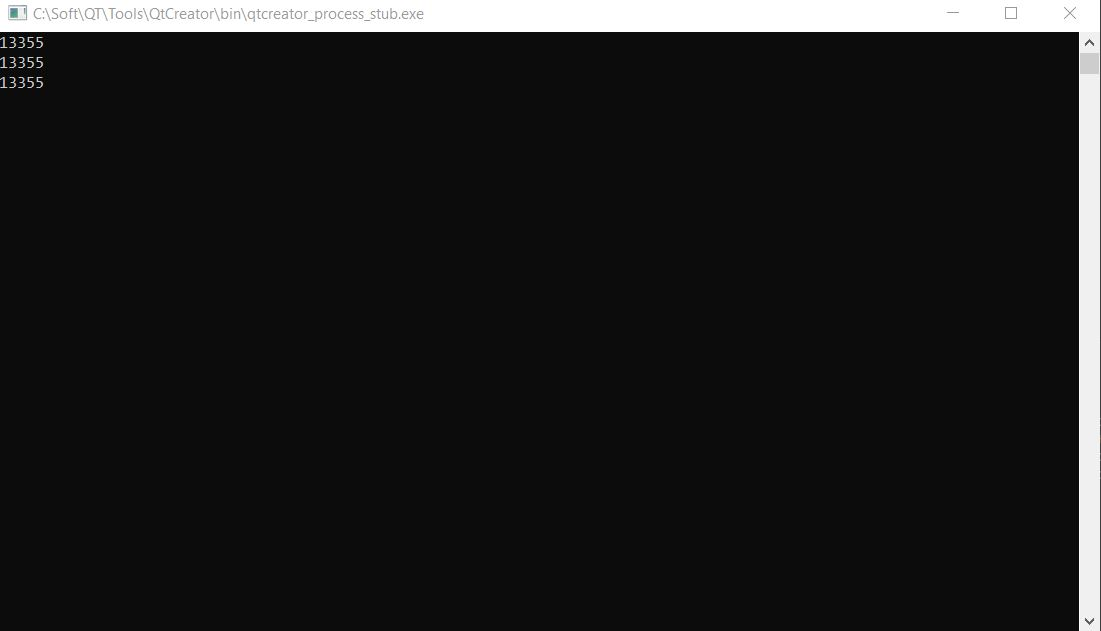
\includegraphics[width=0.7\linewidth]{../Рисунки/screen}
		\caption{Интерфейс программы}
		\label{fig:screen}
	\end{figure}
	
	
\subsection{Листинг}

	В данном подразделе приведен листинг 3 сортировок:
	\begin{enumerate}[1)]
		\item сортировка пузырьком \ref{listing:1};
		\item сортировка вставками \ref{listing:2};
		\item сортировка выборочная. \ref{listing:3};
	\end{enumerate}

	\lstinputlisting[label=listing:1, caption=Сортировка пузырьком]{../../sorts/bubbleSort.cpp}
	\lstinputlisting[label=listing:2, caption=Сортировка вставками]{../../sorts/insertSort.cpp}
	\lstinputlisting[label=listing:3, caption=Сортировка выбором]{../../sorts/selectionSort.cpp}
	
\subsection{Вывод}
	В данном разделе были приведены минимальные системные требования к программе. 
	Указан язык и среда разработки. Приведен образец интерфейса. Располагается листинг.
